\setcounter{equation}{0}
\chapter{Results}

\begin{figure}[h!]
	\begin{center}
		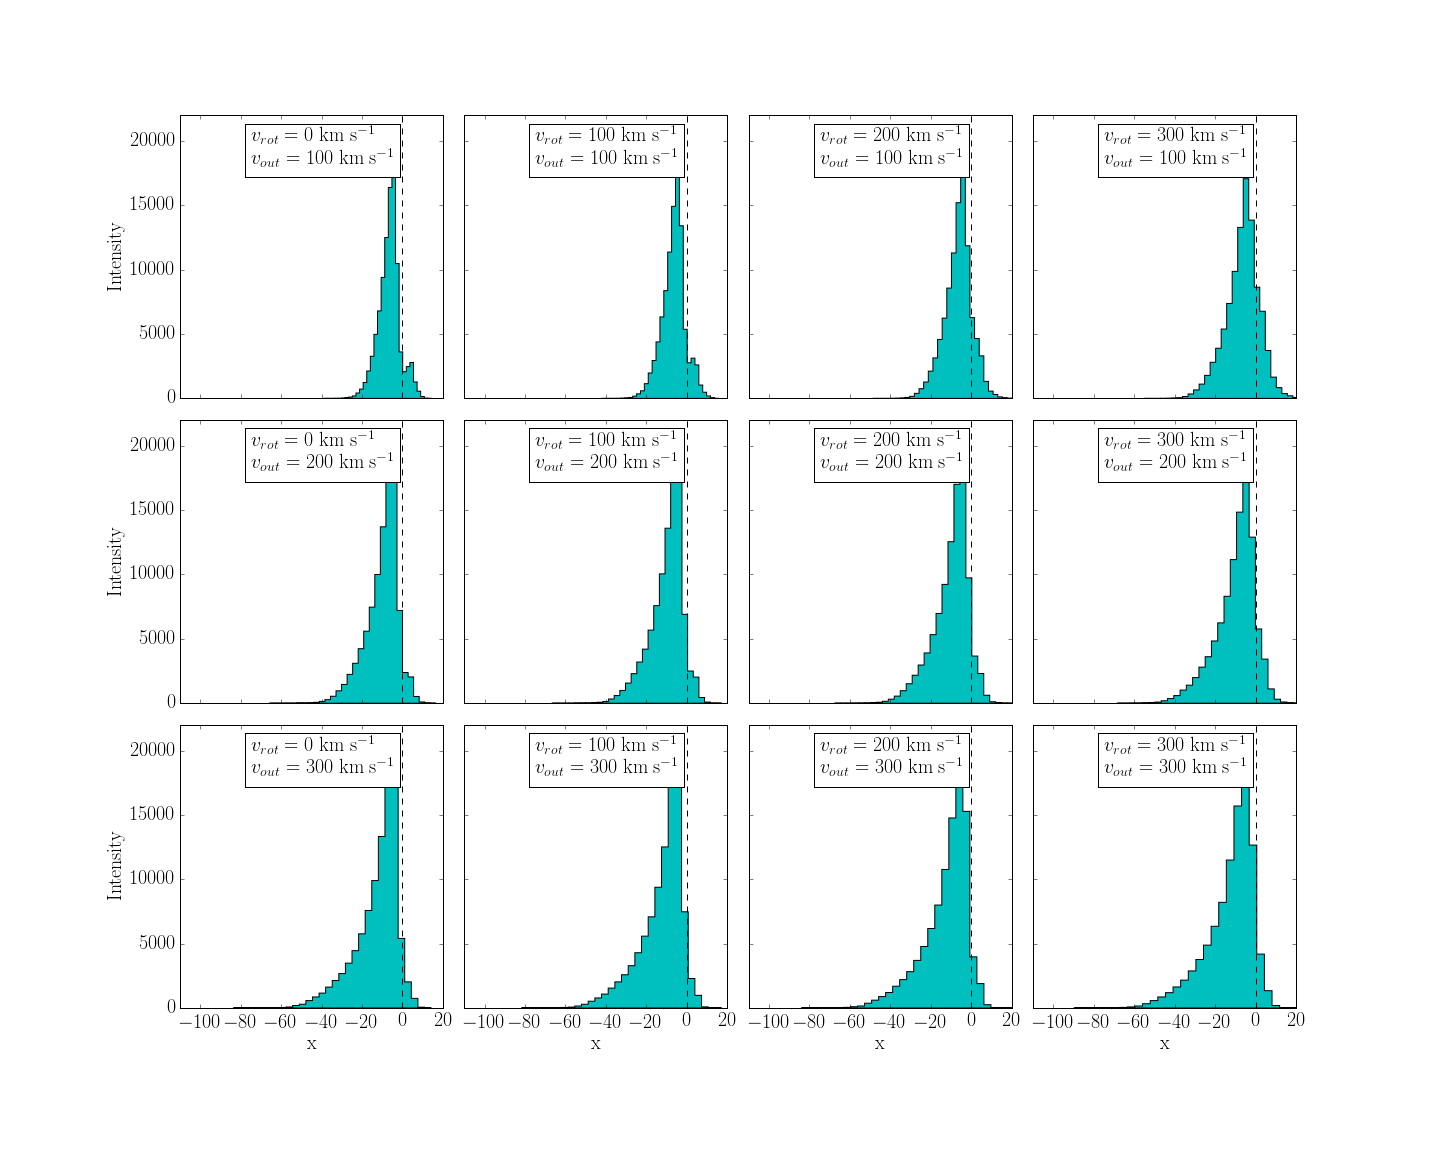
\includegraphics[width=1\textwidth]{./figures/tau10E5.png}
	\end{center}
	\caption{\textbf{\lya profile for \tauh$=10^5$:} With \vrot ranging $0,100,200,300$ \kms and \vout ranging $100,200,300$ \kms.
		\label{fig:tau10E5}}
\end{figure}

\begin{figure}[h!]
	\begin{center}
		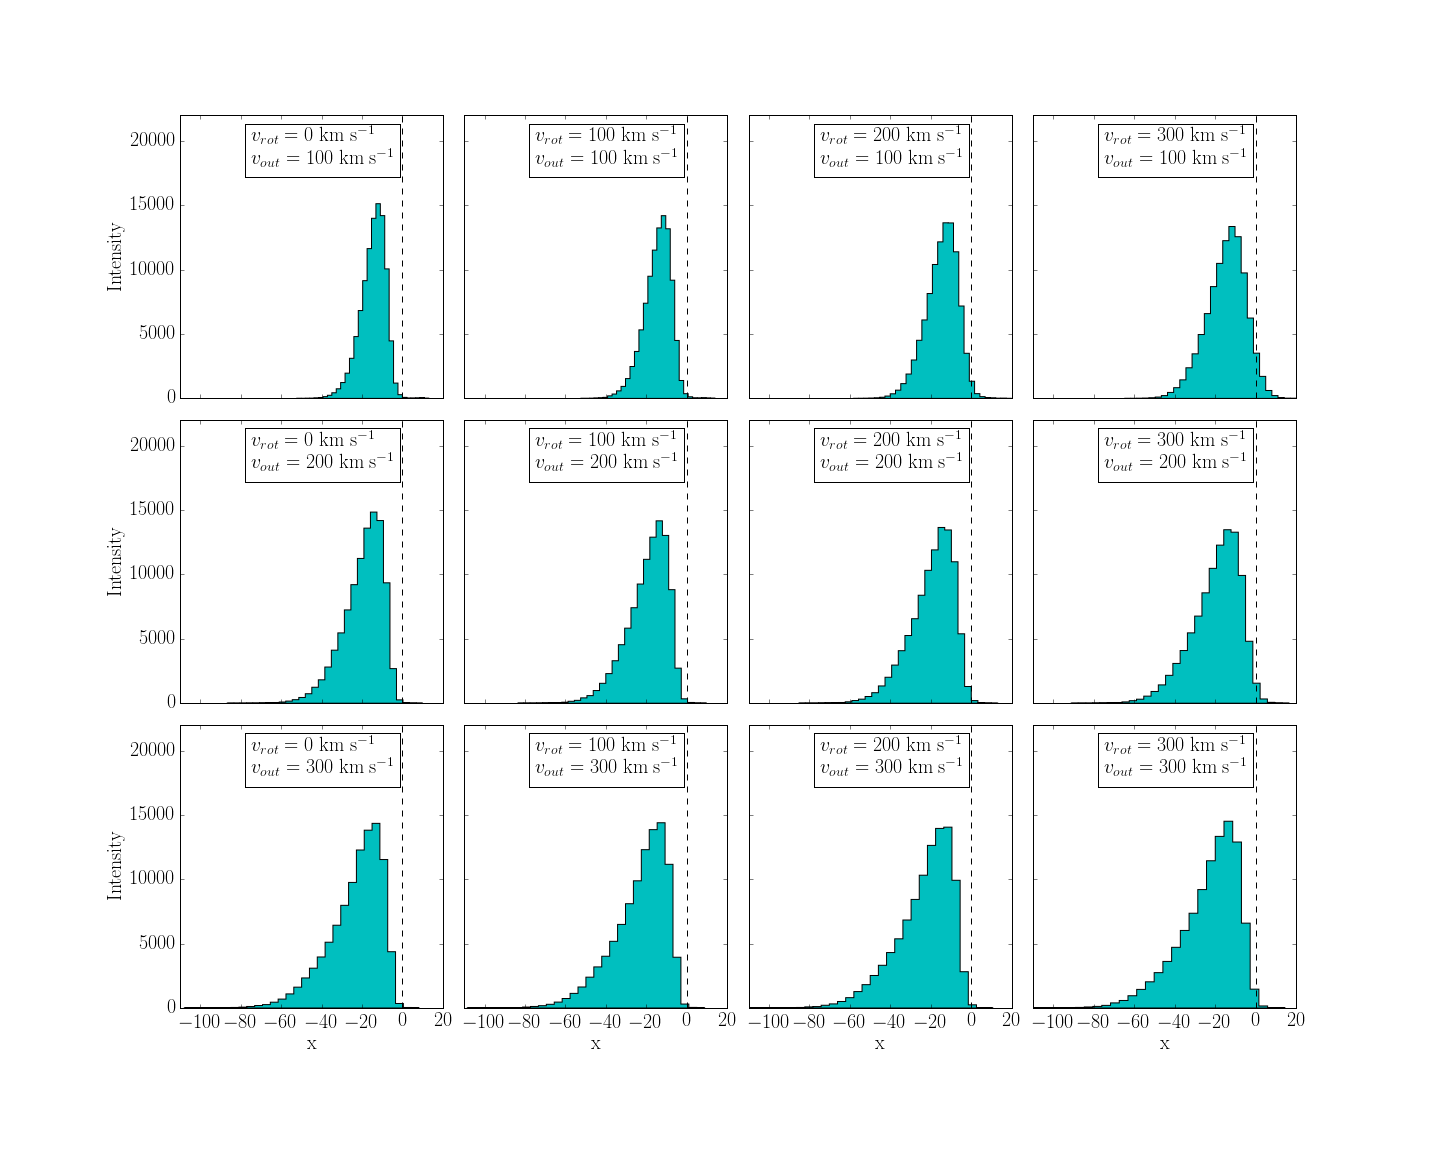
\includegraphics[width=1\textwidth]{./figures/tau10E6.png}
	\end{center}
	\caption{\textbf{\lya profile for \tauh$=10^6$:} With \vrot ranging $0,100,200,300$ \kms and \vout ranging $100,200,300$ \kms.
		\label{fig:tau10E6}}
\end{figure}

\begin{figure}[h!]
	\begin{center}
		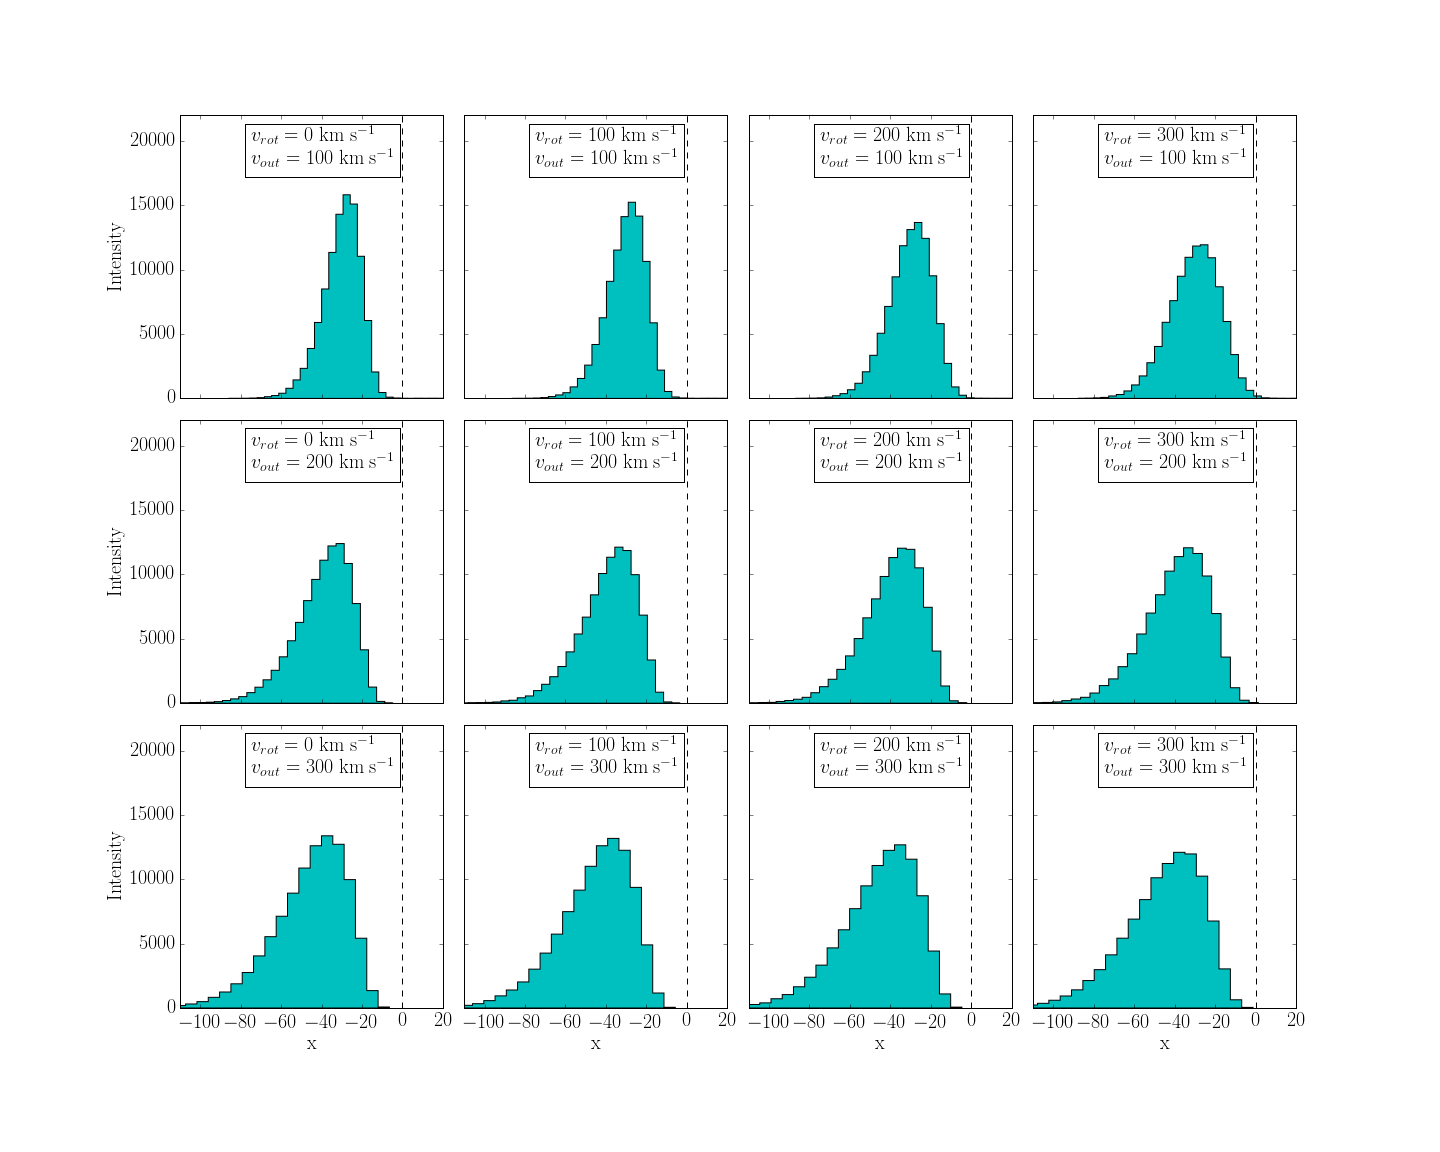
\includegraphics[width=1\textwidth]{./figures/tau10E7.png}
	\end{center}
	\caption{\textbf{\lya profile for \tauh$=10^7$:} With \vrot ranging $0,100,200,300$ \kms and \vout ranging $100,200,300$ \kms.
		\label{fig:tau10E7}}
\end{figure}

\section{Influence of the Galaxy Rotation Velocity: \vrot}


\section{Influence of the Galaxy Outflow Velocity: \vout}


\section{Influence of the Galaxy Optical Depth: \tauh}


\section{Number of Peaks and Peaks Assymetry}